\documentclass{article}
\usepackage{graphicx} 
\usepackage{amsmath}
\usepackage{amssymb}
\usepackage{xcolor}
\usepackage{booktabs}
\usepackage{tabularx}
\usepackage{array}
\usepackage{tikz}
\usepackage{float}
\usepackage[hidelinks]{hyperref}
\usepackage{tocloft} 
\usepackage{graphicx}
\usepackage{subcaption} 
\usepackage{multirow}

\bibliography{BibTex}  % name of your .bib file (NO .bib)
\usepackage[backend=biber,style=trad-plain,sorting=none,doi=false, minbibnames=3, maxbibnames=3, isbn=false,url=false,eprint=false,natbib=true]{biblatex}
\addbibresource{BibTex.bib}

\title{PPP draft}
\author{Mehdi Bakhshi Zadeh}
\date{December 2025}

\begin{document}

\maketitle

\tableofcontents

\section{Introduction}
% TODO: refine motivation + clearly state objectives and success criteria.


\subsection{Project Overview}

This project investigates the numerical solution of the \emph{Gray--Scott reaction--diffusion system}, a coupled set of nonlinear, time-dependent partial differential equations commonly used as a benchmark model for pattern formation in chemical and biological systems. The model describes the evolution of two interacting scalar fields on a two-dimensional square spatial domain with periodic boundary conditions, governed by diffusion and nonlinear reaction terms. The coexistence of diffusive operators and nonlinear reaction dynamics makes the Gray--Scott system a suitable and well-established test case for assessing numerical stability, accuracy, and efficiency.

The spatial discretization of the governing equations is performed using finite difference (FD) methods on a structured two-dimensional grid. Time integration is carried out using explicit time-stepping schemes, which places stability constraints at the center of the numerical analysis. The potentially stiff nature of the reaction terms serves as a motivating factor for studying stability limits and convergence behavior, rather than as a feature addressed through implicit treatment.

The project emphasizes a mathematically consistent formulation of the numerical method, followed by systematic verification through convergence and consistency tests. In addition, attention is given to reproducibility and implementation clarity. Performance-related aspects, including runtime optimization and vectorization, are considered only after the numerical correctness of the method has been established.


\subsection{Motivation and Efficiency Considerations}

Although the Gray--Scott model is conceptually simple, its numerical solution becomes computationally demanding when fine spatial and temporal resolutions are required to accurately resolve emerging patterns. In particular, explicit time integration schemes impose restrictive stability conditions that directly link the admissible time step size to the spatial grid spacing. As the grid is refined, the number of required time steps increases rapidly, leading to a significant growth in computational cost.

For diffusion operators discretized with finite differences on structured grids, the resulting linear operators exhibit a highly regular sparsity pattern. In the baseline implementation considered in this work, the discrete Laplacian is assembled explicitly as a sparse matrix using Kronecker products of one-dimensional second-derivative operators. This formulation preserves the mathematical structure of the five-point finite-difference stencil and enables efficient matrix--vector products while maintaining clarity and ease of verification.
% TODO (after implementing variant): update this paragraph to describe
% the stencil-based three-vector diffusion operator variant and compare
% it with the sparse-matrix baseline in terms of memory and performance.


Efficiency is therefore treated as a secondary objective that builds upon a fully verified and stable numerical formulation.

\subsection{Objectives and Definition of Success}

The primary objective of this project is to develop a correct, stable, and verifiable finite difference solver for the two-dimensional Gray--Scott equations. Success is defined using the following measurable criteria:

\begin{itemize}
    \item The governing equations, initial conditions, and boundary conditions are clearly stated and correctly discretized using finite difference methods on a structured grid.
    \item The numerical scheme is shown to be consistent through operator-level tests, including verification of the discrete Laplacian and basic time-step refinement checks.
    \item Stability restrictions associated with explicit time integration are derived and discussed, and their qualitative implications are confirmed through numerical experiments.
    \item A clear and verifiable sparse-matrix formulation of the diffusion operator is implemented as the baseline solver; alternative stencil-based formulations are identified as future extensions.
    \item Numerical results are validated through internal consistency checks and qualitative comparison with known Gray--Scott pattern formation behavior reported in the literature.
\end{itemize}

% TODO: update objectives after implementing additional solver variants.

Optional performance comparisons may be included at later stages of the project, but only after numerical correctness and verification have been conclusively demonstrated.

\section{Mathematical Model}
% TODO: move/merge the Gray--Scott PDE subsection here and finalize citations.


\subsection{Gray--Scott Reaction--Diffusion System}

Let $\Omega \subset \mathbb{R}^2$ be a two-dimensional spatial domain with coordinates
$(x,y)$, and let $t \in [0,T]$ denote time. We consider two scalar fields
$u(x,y,t)$ and $v(x,y,t)$, representing the (dimensionless) concentrations of two chemical
species $U$ and $V$.

The Gray--Scott model is the coupled reaction--diffusion system
\begin{align}
\frac{\partial u}{\partial t} &= D_u \nabla^2 u \;-\; u v^2 \;+\; F(1-u),
\\
\frac{\partial v}{\partial t} &= D_v \nabla^2 v \;+\; u v^2 \;-\; (F+k)\,v,
\end{align}
where $D_u, D_v > 0$ are diffusion coefficients, and $F>0$ and $k>0$ are the feed and kill
rates, respectively. This formulation is standard for the Gray--Scott system and is widely used
in studies of reaction--diffusion pattern formation~\cite{pearson1993}.


\paragraph{Interpretation of terms.}
The Laplacian terms $D_u \nabla^2 u$ and $D_v \nabla^2 v$ model diffusion (spatial
spreading/smoothing). The nonlinear reaction term $u v^2$ is autocatalytic: it consumes $u$
and produces $v$ (hence $-uv^2$ in the $u$-equation and $+uv^2$ in the $v$-equation).
The feed term $F(1-u)$ replenishes $u$ toward the background value $u=1$, while the removal
term $(F+k)v$ depletes $v$ through outflow ($F$) and an additional decay mechanism ($k$).

\paragraph{Boundary conditions.}
In the baseline implementation considered in this work, periodic boundary conditions are imposed
in both spatial directions for both $u$ and $v$. Periodicity is enforced by wrapping grid indices
across domain boundaries in the finite-difference discretization. This choice simplifies the
numerical implementation, avoids artificial boundary effects, and is commonly adopted in studies
of Gray--Scott pattern formation.
% TODO: extend boundary-condition support (e.g., Neumann) if required in future variants.


\paragraph{Initial conditions.}
Initial conditions $u(x,y,0)=u_0(x,y)$ and $v(x,y,0)=v_0(x,y)$ are prescribed, typically as
a nearly homogeneous state with a localized perturbation (``seed'') to trigger pattern formation.

\subsection*{Typical Parameter Sets}

Unless stated otherwise, the diffusion coefficients are chosen following
the standard parameterization used by Pearson~\cite{pearson1993}, namely
\[
D_u = 2\times 10^{-5}, \qquad D_v = 1\times 10^{-5}.
\]
Only the ratio $D_u/D_v$ is essential for the qualitative pattern-forming
behavior of the Gray--Scott system; absolute values primarily affect the
temporal and spatial scales of the dynamics.


Table~\ref{tab:gs-parameters} lists representative values of the feed rate $F$
and kill rate $k$ that are known to generate distinct qualitative pattern
regimes in two-dimensional simulations, provided suitable initial perturbations
are applied. The parameter sets listed below are representative values commonly used
in the literature for qualitative exploration of pattern regimes and are
not intended to exhaustively characterize the full parameter space.


\begin{table}[h!]
\centering
\caption{Representative Gray--Scott parameter sets and associated pattern regimes.}
\label{tab:gs-parameters}
\begin{tabular}{c c c l}
\hline
Regime & $F$ & $k$ & Qualitative behavior \\ \hline
Spots & 0.035 & 0.060 & Isolated spot patterns \\
Spots & 0.030 & 0.062 & Dense spot replication \\
Stripes (maze) & 0.026 & 0.051 & Labyrinthine stripe patterns \\
Mixed / chaotic & 0.022 & 0.051 & Transitional or mixed structures \\ \hline
\end{tabular}
\end{table}

In this work, selected parameter sets are used to demonstrate the behavior
of the numerical solver and to enable qualitative comparison with reference
studies such as Pearson~\cite{pearson1993, sims1994}.
 The exact morphology depends on the spatial resolution, time step,
boundary conditions, and initial perturbations.

\section{Numerical Methods}
% TODO: include spatial discretization, time stepping, and stability discussion here.


\subsection{Spatial Discretization (Finite Differences)}

The two-dimensional computational domain $\Omega = [0,L_x)\times[0,L_y)$ is discretized using a
structured Cartesian grid with $N_x$ grid points in the $x$-direction and $N_y$ grid points in
the $y$-direction. The grid coordinates are defined as
\[
x_i = i\,h_x,\quad i=0,\dots,N_x-1, 
\qquad
y_j = j\,h_y,\quad j=0,\dots,N_y-1,
\]
where uniform spacings $h_x=L_x/N_x$ and $h_y=L_y/N_y$ are used. The right boundaries are excluded to avoid duplicate grid points under periodic boundary conditions. 
For non-periodic boundary conditions (Dirichlet or Neumann), boundary nodes are treated explicitly 
during the time-stepping procedure, while the interior discretization remains unchanged. For any grid function
$u(x,y,t)$, the discrete value at $(x_i,y_j)$ is denoted by $u_{i,j}(t)$.
This finite-difference discretization on a uniform periodic grid follows the numerical
approach adopted in Pearson’s original study of the Gray--Scott system, where simplicity
and computational efficiency were prioritized to enable extensive parameter exploration.


\paragraph{2D Laplacian and five-point stencil.}
The Laplacian operator is given by
\[
\nabla^2 u = \frac{\partial^2 u}{\partial x^2} + \frac{\partial^2 u}{\partial y^2}.
\]
Using second-order central finite differences, the second derivatives at $(x_i,y_j)$ are
approximated by
\begin{align}
\frac{\partial^2 u}{\partial x^2}(x_i,y_j)
&\approx \frac{u_{i+1,j}-2u_{i,j}+u_{i-1,j}}{h_x^2},\\
\frac{\partial^2 u}{\partial y^2}(x_i,y_j)
&\approx \frac{u_{i,j+1}-2u_{i,j}+u_{i,j-1}}{h_y^2}.
\end{align}
Combining these expressions yields the standard five-point approximation of the Laplacian:
\begin{equation}
(\nabla^2 u)_{i,j} \approx
\frac{u_{i+1,j}+u_{i-1,j}-2u_{i,j}}{h_x^2}
+
\frac{u_{i,j+1}+u_{i,j-1}-2u_{i,j}}{h_y^2}.
\label{eq:laplacian_5pt}
\end{equation}
An identical stencil is applied to the concentration field $v$.

\paragraph{Order of accuracy.}
The central-difference approximations used above have a truncation error proportional to
$h_x^2$ and $h_y^2$. Consequently, the discrete Laplacian~\eqref{eq:laplacian_5pt} is
\emph{second-order accurate} in space for sufficiently smooth solutions at interior grid points.
For periodic boundary conditions, this second-order accuracy extends uniformly over the entire
domain due to the translational invariance of the stencil. In the case of Dirichlet or Neumann
boundary conditions, the interior discretization remains second-order accurate, while boundary
values are imposed strongly after each time update using one-sided difference relations for
Neumann conditions. Although the one-sided boundary treatment is formally first-order accurate
at the boundary itself, the overall spatial convergence of the scheme remains second-order for
smooth solutions, since boundary nodes constitute a lower-dimensional subset of the grid.
While higher-order spatial discretizations are possible, the present second-order scheme provides
a robust and well-understood baseline suitable for verification and consistent with the
Pearson-style reaction--diffusion simulations considered in this work.


\paragraph{Indexing strategy (2D to 1D mapping).}
For implementation and linear-algebra formulations, the two-dimensional grid values
$u_{i,j}$ are stored as one-dimensional vectors using MATLAB's column-major ordering.
Specifically, the mapping
\begin{equation}
k = j + (i-1)N_y,
\qquad i=1,\dots,N_x,\;\; j=1,\dots,N_y,
\label{eq:column_major_mapping}
\end{equation}
is employed, such that the $y$-index varies fastest in memory. With this convention,
neighboring grid points in the $y$-direction correspond to indices $k\pm 1$, while neighbors
in the $x$-direction correspond to indices $k\pm N_y$. This mapping is consistent with
MATLAB’s internal memory layout and simplifies the construction of sparse finite-difference
operators.

\paragraph{Stencil illustration.}
The five-point stencil couples each grid point $(i,j)$ to its four axial neighbors:
\begin{figure}[H]
  \centering
  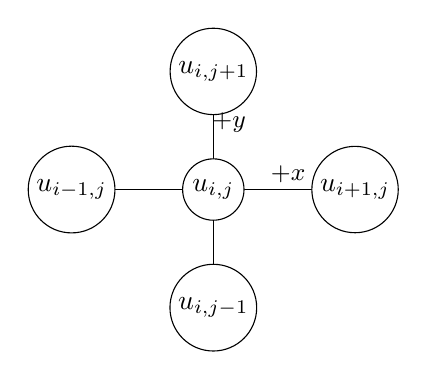
\begin{tikzpicture}[scale=1.0, line cap=round, line join=round]
    % Nodes
    \node[circle, draw, inner sep=2pt] (C) at (0,0) {$u_{i,j}$};
    \node[circle, draw, inner sep=2pt] (N) at (0,1.5) {$u_{i,j+1}$};
    \node[circle, draw, inner sep=2pt] (S) at (0,-1.5) {$u_{i,j-1}$};
    \node[circle, draw, inner sep=2pt] (E) at (1.8,0) {$u_{i+1,j}$};
    \node[circle, draw, inner sep=2pt] (W) at (-1.8,0) {$u_{i-1,j}$};

    % Connections
    \draw[-] (C) -- (N);
    \draw[-] (C) -- (S);
    \draw[-] (C) -- (E);
    \draw[-] (C) -- (W);

    % Optional: small labels for direction
    \node at (0.95, 0.2) {\small $+x$};
    \node at (0.2, 0.85) {\small $+y$};
  \end{tikzpicture}
  \caption{Five-point finite-difference stencil for the 2D Laplacian at grid point $(i,j)$.}
  \label{fig:five_point_stencil}
\end{figure}


\subsection{Time Discretization (Explicit Euler) and Stability}

Let $\Delta t>0$ denote the time-step size and define discrete times $t^n = n\Delta t$.
Numerical approximations at time $t^n$ are denoted by
$u_{i,j}^n \approx u(x_i,y_j,t^n)$ and
$v_{i,j}^n \approx v(x_i,y_j,t^n)$.
Time integration of the Gray--Scott system is performed using a first-order explicit Euler
scheme. This choice mirrors the numerical approach adopted by Pearson~\cite{pearson1993}, where
explicit Euler time stepping was employed to enable efficient large-scale simulations and
qualitative exploration of pattern-forming regimes.
 The fully discrete update equations are given by
\begin{align}
u_{i,j}^{n+1} &=
u_{i,j}^{n} + \Delta t\Big(
D_u (\nabla_h^2 u)_{i,j}^{n}
- u_{i,j}^{n} (v_{i,j}^{n})^2
+ F(1-u_{i,j}^{n})
\Big), \label{eq:Euler_u} \\
v_{i,j}^{n+1} &=
v_{i,j}^{n} + \Delta t\Big(
D_v (\nabla_h^2 v)_{i,j}^{n}
+ u_{i,j}^{n} (v_{i,j}^{n})^2
- (F+k)v_{i,j}^{n}
\Big), \label{eq:Euler_v}
\end{align}
where $\nabla_h^2$ denotes the discrete Laplacian operator constructed using second-order
central finite differences. On a uniform Cartesian grid with spacings $h_x$ and $h_y$, it is defined as
\begin{equation}
(\nabla_h^2 w)_{i,j}^{n} =
\frac{w_{i+1,j}^{n}-2w_{i,j}^{n}+w_{i-1,j}^{n}}{h_x^2}
+
\frac{w_{i,j+1}^{n}-2w_{i,j}^{n}+w_{i,j-1}^{n}}{h_y^2}.
\label{eq:laplacian_fd_time}
\end{equation}


\paragraph{Stability considerations.}
To assess stability, it is instructive to consider the diffusion equation
$w_t = D\nabla^2 w$ obtained by neglecting reaction terms. After spatial discretization,
this leads to a linear system with real, negative eigenvalues. Applying explicit Euler to
a single eigenmode yields the stability condition $|1+\Delta t\,\lambda|\le 1$.
For the two-dimensional five-point Laplacian, the most restrictive eigenvalues scale on the
order of $-h^{-2}$, implying a diffusion-limited timestep restriction of the form
$\Delta t \lesssim h^2/D$.
In the context of the present work, this stability restriction is treated as a practical
guideline rather than a sharp bound, since the primary objective is to obtain stable and
qualitatively correct solutions rather than to maximize timestep size.


\paragraph{Practical timestep selection.}
On sufficiently fine grids, stability of the explicit Euler method is typically dominated
by the diffusion terms, leading to the well-known scaling
$\Delta t = \mathcal{O}(h^2)$. In practice, a conservative timestep can be selected based on the largest diffusion coefficient
$D_{\max}=\max(D_u,D_v)$ and the grid spacings. A commonly used sufficient condition for explicit
Euler stability of the diffusion terms on a 2D grid is
\begin{equation}
\Delta t \le \eta\,
\frac{1}{2D_{\max}\left(\frac{1}{h_x^2}+\frac{1}{h_y^2}\right)},
\qquad 0<\eta<1,
\label{eq:dt_choice}
\end{equation}
which reduces to $\Delta t = \mathcal{O}(h^2/D_{\max})$ when $h_x=h_y=h$.

In this work, a conservative value of $\eta$ is adopted to prioritize numerical stability
and correctness, in contrast to the more aggressive timestep choices sometimes used in
purely exploratory studies.
 The adequacy of this timestep choice is further confirmed through numerical
verification tests presented in Section~\ref{sec:verification}.

\section{Verification and Validation}
% TODO (FINAL CHECK BEFORE SUBMISSION):
% Ensure that all verification tests described in this section
% have been fully implemented and executed.
% Remove or update any items that are not completed.

\subsection{Verification Strategy}

Verification addresses the question: \emph{does the implementation correctly solve the
discretized Gray--Scott equations?} The goal is to confirm the expected convergence behavior
in space and time, and to detect potential implementation errors (such as incorrect indexing,
boundary handling, or operator application) using quantitative error measures and clearly
defined pass/fail criteria.

\paragraph{Error norms.}
For a grid function $w_{i,j}$ and an exact or reference solution $w^{*}_{i,j}$, we define the
pointwise error $e_{i,j} = w_{i,j} - w^{*}_{i,j}$ and compute the following norms:
\begin{align}
\|e\|_\infty &= \max_{i,j} |e_{i,j}|, \\
\|e\|_2 &= \left( h_x h_y \sum_{i,j} e_{i,j}^2 \right)^{1/2},
\end{align}
with both norms evaluated independently for the variables $u$ and $v$.

\paragraph{Observed order of convergence.}
Under grid refinement, the observed spatial order of convergence is estimated using errors
$E(h)$ and $E(h/2)$ as
\[
p_{\text{space}} = \log_2\!\left(\frac{E(h)}{E(h/2)}\right).
\]
Similarly, under time-step refinement, the observed temporal order is computed from errors
$E(\Delta t)$ and $E(\Delta t/2)$ as
\[
p_{\text{time}} = \log_2\!\left(\frac{E(\Delta t)}{E(\Delta t/2)}\right).
\]

\paragraph{Pass/fail criteria.}
Verification tests are considered successful if the observed numerical behavior
is consistent with the formal accuracy of the underlying schemes and with the
nature of the test problem. For isolated spatial operators verified using
manufactured solutions, second-order spatial accuracy is expected for the
finite-difference discretization of the Laplacian. For time integration using
explicit Euler, first-order temporal accuracy is expected.

For full Gray--Scott simulations, which are nonlinear and capable of pattern
formation, strict second-order convergence in field norms is not enforced.
Instead, grid refinement tests are interpreted as consistency checks: solutions
must exhibit stable behavior and decreasing differences under refinement.
Additional sanity checks include finite solution values (absence of NaNs or
Infs) and stable behavior under the chosen timestep.


\begin{table}[!t]
\centering
\caption{Verification tests used to assess correctness, stability, and convergence of the
numerical solver.}
\label{tab:verification_plan}
\small
\renewcommand{\arraystretch}{1.2}
\begin{tabularx}{\textwidth}
{>{\raggedright\arraybackslash}p{3.2cm}
 >{\raggedright\arraybackslash}X
 >{\raggedright\arraybackslash}X}
\toprule
\textbf{Test} & \textbf{Purpose} & \textbf{Expected result / Pass--Fail criterion} \\
\midrule
Grid refinement (Gray--Scott) &
Assess solution consistency under spatial refinement for the full nonlinear system. &
Differences in $u$ and $v$ decrease monotonically under grid refinement.
Observed convergence rates may be below second order due to explicit Euler
time integration and nonlinear pattern sensitivity.
\textbf{Pass} if refinement leads to decreasing errors and stable behavior. \\

Time-step halving &
Confirm temporal convergence of explicit Euler integration. &
With fixed fine spatial resolution, decreasing $\Delta t$ yields
$p_{\text{time}} \approx 1$ for both variables and both norms.
\textbf{Pass} if $p_{\text{time}} \ge 0.95$. \\

Manufactured solution (MMS) &
End-to-end verification using an exact smooth solution enforced via source terms. &
Under combined spatial and temporal refinement, recover
$p_{\text{space}} \approx 2$ and $p_{\text{time}} \approx 1$.
\textbf{Pass} if thresholds above are satisfied. \\
\bottomrule
\end{tabularx}
\end{table}

\paragraph{Test organization.}
All verification tests are implemented as separate scripts in the \texttt{/tests} directory
to keep verification independent from the main simulation driver. Each test reports error
norms, observed convergence behavior where applicable, and clear diagnostic messages
indicating success or failure. Optional plots, such as log--log error curves or difference
fields, are saved to the \texttt{/figures} directory. All verification figures are generated by automated test scripts and saved together
with associated parameter metadata in \texttt{.mat} files to support reproducibility.



\subsection{Verification (Baseline)}
\label{sec:verification}

A fixed reference implementation is established and verified prior to any performance-oriented modifications.
All subsequent comparisons are conducted against this reference solver, which remains numerically unchanged throughout the study.
The purpose of the baseline verification is to confirm correctness of both individual numerical components and their coupled behavior in the full Gray--Scott system.

First, the discrete Laplacian operator is verified independently of the reaction--diffusion model.
For periodic boundary conditions, the Laplacian of a constant field must vanish; this property is confirmed numerically to machine precision.
In addition, symmetry of the discrete operator is checked, ensuring consistency of the finite-difference stencil and correctness of the Kronecker-based assembly.

Second, a time-step halving smoke test is performed for the full Gray--Scott system using explicit Euler time integration.
Simulations are run to the same final time using time steps $\Delta t$ and $\Delta t/2$, and the resulting solutions are compared.
The difference between the two solutions remains small, smooth, and spatially localized, indicating stable and consistent temporal integration.
Figure~\ref{fig:timestep_halving} illustrates the spatial distribution of the difference in the $v$ field at the final time.

Finally, a manufactured-solution testing scaffold is introduced to enable rigorous verification of the spatial discretization using exact smooth solutions.
This framework allows independent assessment of the discrete operators without interference from nonlinear reaction terms.
Full manufactured-solution verification results are presented in Section~\ref{sec:mms}, where second-order spatial convergence of the discrete Laplacian is confirmed.

All verification tests pass within prescribed tolerances, and the corresponding figures and metadata are saved automatically to disk.
This verified reference implementation serves as the numerical baseline for all performance and solver-variant comparisons presented later in the report.

\begin{figure}[ht]
  \centering
  \includegraphics[width=0.6\textwidth]{figures/timestep_halving_diffV.png}
  \caption{Difference in the $v$ field between simulations using $\Delta t$ and $\Delta t/2$
at the same final time. Parameters: $N=128$, $T=50$, $\Delta t=0.2$. The localized difference
pattern demonstrates stable and consistent explicit Euler time integration.}
  \label{fig:timestep_halving}
\end{figure}

\subsection{Manufactured Solution Verification}
\label{sec:mms}

The method of manufactured solutions (MMS) is used to rigorously verify the
spatial discretization independently of the nonlinear Gray--Scott dynamics.
Smooth analytical target functions $u^*(x,y,t)$ and $v^*(x,y,t)$ are prescribed,
and corresponding source terms are derived such that the forced system is
satisfied exactly by the manufactured solution.

Periodic trigonometric functions are selected to match the periodic boundary
conditions of the solver, which allows the analytic Laplacians
$\Delta u^*$ and $\Delta v^*$ to be computed in closed form. The discrete
Laplacian operator is applied to the manufactured fields and compared directly
against the analytic expressions. Errors are measured in a weighted discrete
$L^2$ norm under grid refinement.

Table~\ref{tab:mms_operator} reports the $L^2$ errors of the discrete Laplacian
applied to the manufactured solution for increasing grid resolutions. The
observed convergence orders are computed from successive grid refinements.

\begin{table}[H]
\centering
\caption{MMS verification of the discrete Laplacian operator. Reported are
$L^2$ errors and observed spatial convergence orders.}
\label{tab:mms_operator}
\small
\renewcommand{\arraystretch}{1.2}
\begin{tabular}{cccc}
\toprule
Grid size $N$ & $\|L u^* - \Delta u^*\|_{L^2}$ &
$\|L v^* - \Delta v^*\|_{L^2}$ & Observed order \\
\midrule
32  & $8.609\times10^{-1}$ & $8.609\times10^{-1}$ & -- \\
64  & $2.169\times10^{-1}$ & $2.169\times10^{-1}$ & 1.99 \\
128 & $5.434\times10^{-2}$ & $5.434\times10^{-2}$ & 1.99 \\
256 & $1.359\times10^{-2}$ & $1.359\times10^{-2}$ & 2.00 \\
\bottomrule
\end{tabular}
\end{table}

The results demonstrate clear second-order spatial convergence of the discrete
Laplacian operator, with observed orders very close to the theoretical value of
two. This confirms that the finite-difference stencil, indexing, and boundary
handling are implemented correctly. Because this test isolates the spatial
operator, it provides an unambiguous verification of spatial accuracy that is
not influenced by time integration or nonlinear reaction terms.


\begin{figure}[H]
  \centering
  \includegraphics[width=0.65\textwidth]{figures/verification/mms_operator_convergence.png}
  \caption{Manufactured-solution verification of the discrete Laplacian operator.
Weighted $L^2$ errors are shown for grid sizes $N=\{32,64,128,256\}$.
The log--log slope is approximately two, indicating second-order spatial accuracy.}
  \label{fig:mms_operator_convergence}
\end{figure}

\subsection{Grid Refinement Consistency (Gray--Scott)}
\label{sec:grid-refinement}

A grid refinement study is performed for the full, unforced Gray--Scott
reaction--diffusion system to assess solution consistency under increasing
spatial resolution. In contrast to the MMS tests, no analytic reference
solution exists for the Gray--Scott equations, and verification must rely on
comparisons between numerical solutions on different grids.

Simulations are conducted on grids with $N \in \{64,128,256,512\}$ up to a short
final time $T=1$. The explicit Euler method is used for time integration.
To reduce the influence of time-discretization errors while remaining consistent
with the proposed numerical scheme, the timestep is scaled proportionally to the
square of the grid spacing, $dt \propto h^2$. The solution on the finest grid
($N=512$) is treated as a reference and interpolated onto coarser grids using
bicubic interpolation. Weighted discrete $L^2$ differences are computed for both
solution variables.

Table~\ref{tab:grayscott_refinement} summarizes the measured $L^2$ differences
between the coarse-grid solutions and the interpolated finest-grid reference.

\begin{table}[H]
\centering
\caption{Gray--Scott grid refinement study. Reported are weighted $L^2$
differences with respect to the finest-grid ($N=512$) reference solution at
final time $T=1$.}
\label{tab:grayscott_refinement}
\small
\renewcommand{\arraystretch}{1.2}
\begin{tabular}{ccc}
\toprule
Grid size $N$ & $\|u_N - u_{512}\|_{L^2}$ & $\|v_N - v_{512}\|_{L^2}$ \\
\midrule
64  & $1.647\times10^{-1}$ & $8.486\times10^{-2}$ \\
128 & $7.766\times10^{-2}$ & $4.089\times10^{-2}$ \\
256 & $3.030\times10^{-2}$ & $1.694\times10^{-2}$ \\
\bottomrule
\end{tabular}
\end{table}

Using these values, the observed convergence rates computed from all available
coarse grids are $p_u = 1.247$ and $p_v = 1.184$. While these rates are below the
formal second-order accuracy of the spatial discretization, the results exhibit
a clear monotonic decrease in the differences as the grid is refined, indicating
improved solution consistency.

\paragraph{Challenges and interpretation.}
Interpreting grid refinement results for the Gray--Scott system is inherently
challenging. The equations are nonlinear and capable of pattern formation, which
makes the solution sensitive to small perturbations. Minor differences in grid
resolution or time stepping can lead to slight phase shifts in emerging
structures. Although such shifts may be visually insignificant, they can produce
relatively large differences in global $L^2$ norms.

In addition, the explicit Euler method is first-order accurate in time, and
temporal errors accumulate over many time steps. Even with the timestep scaled
as $dt \propto h^2$, time-integration errors interact with nonlinear dynamics
and prevent the solver from entering a clean second-order spatial asymptotic
regime. Finally, interpolating the fine-grid reference solution onto coarser
grids introduces additional approximation error.

For these reasons, the grid refinement study is interpreted as a consistency
check rather than a strict convergence proof. When considered together with the
MMS-based operator verification, the results provide strong evidence that the
spatial discretization is correctly implemented and that the full solver behaves
consistently under grid refinement.


\begin{figure}[H]
  \centering
  \includegraphics[width=0.65\textwidth]{figures/verification/grayscott_grid_refinement.png}
  \caption{Grid refinement consistency study for the Gray--Scott system using explicit
Euler time integration. Differences with respect to the finest-grid reference
($N=512$) are shown for $N=\{64,128,256\}$ at final time $T=1.0$, with the timestep
scaled as $\Delta t \propto h^2$ (baseline $\Delta t_0=0.01$). Differences decrease
monotonically as the grid is refined.}
  \label{fig:grayscott_grid_refinement}
\end{figure}

\subsection{Time-step Refinement and Temporal Convergence}
\label{sec:verification_time}

While basic time-step sensitivity is addressed as part of the baseline
verification, a dedicated time-step refinement study is conducted here to
quantitatively verify the temporal accuracy and stability of the explicit
Euler time integration used throughout this project.

\paragraph{Test setup.}
All simulations are performed on a fixed spatial grid with
$N_x = N_y = 128$ and periodic boundary conditions. A stable baseline time
step $\Delta t$ is selected, and the Gray--Scott system is integrated to the
same final time $T = 50$ using three different time steps:
\[
\Delta t,\quad \Delta t/2,\quad \Delta t/4.
\]
The spatial discretization is held constant in order to isolate temporal
discretization effects.

\paragraph{Comparison methodology.}
In the absence of an exact time-dependent solution for the Gray--Scott
system, temporal convergence is assessed using a Richardson-style approach
based on successive solution differences. Let $v_{\Delta t}$,
$v_{\Delta t/2}$, and $v_{\Delta t/4}$ denote the numerical solutions for the
$v$ field at final time $T$. The following differences are computed:
\[
d_{12} = \| v_{\Delta t} - v_{\Delta t/2} \|, \qquad
d_{24} = \| v_{\Delta t/2} - v_{\Delta t/4} \|.
\]
Both the discrete $L^2$ norm and the $L^\infty$ norm are evaluated. An
observed temporal convergence order is then estimated as
\[
p_{\text{time}} = \log_2\!\left(\frac{d_{12}}{d_{24}}\right).
\]

\paragraph{Expected behavior.}
The explicit Euler method is first-order accurate in time. Therefore,
halving the time step is expected to approximately halve the temporal error,
leading to an observed convergence rate $p_{\text{time}} \approx 1$.

\paragraph{Observed results.}
Table~\ref{tab:timestep_convergence} summarizes the measured successive
differences and observed convergence rates. In both error norms, the
differences decrease consistently under time-step refinement, and the
measured convergence orders are very close to one.

\begin{table}[ht]
\centering
\caption{Time-step refinement results for explicit Euler integration
($N_x = N_y = 128$, $T = 50$).}
\label{tab:timestep_convergence}
\small
\renewcommand{\arraystretch}{1.2}
\begin{tabular}{lccc}
\toprule
Norm & $d_{12}$ & $d_{24}$ & Observed order $p_{\text{time}}$ \\
\midrule
$L^2$ &
$4.244\times 10^{-5}$ &
$2.115\times 10^{-5}$ &
$1.005$ \\
$L^\infty$ &
$6.105\times 10^{-4}$ &
$3.046\times 10^{-4}$ &
$1.003$ \\
\bottomrule
\end{tabular}
\end{table}

Figure~\ref{fig:timestep_convergence} presents a log--log plot of the
successive differences versus the time step size. The near-linear behavior
with slope approximately equal to one further confirms first-order temporal
accuracy.

\begin{figure}[ht]
  \centering
  \includegraphics[width=0.6\textwidth]{figures/verification/timestep_convergence.png}
  \caption{Time-step refinement for explicit Euler integration on a fixed grid
($N=128$, $T=50$). Successive differences between solutions using
$\Delta t=\{0.2,0.1,0.05\}$ decrease linearly with $\Delta t$, indicating first-order
temporal convergence.}
  \label{fig:timestep_convergence}
\end{figure}

\paragraph{Discussion and challenges.}
The results demonstrate that the explicit Euler method exhibits the expected
first-order temporal convergence when applied to the Gray--Scott system.
Ensuring that spatial discretization errors do not contaminate the temporal
convergence measurement is a key challenge in this test. This is addressed by
fixing a sufficiently fine spatial grid and comparing only successive
time-step refinements at the same final time.

Overall, the observed behavior provides strong verification evidence for the
correctness and stability of the time integration scheme used in this work
and complements the spatial and manufactured-solution verification results
presented in the preceding sections.

\subsection{Boundary Condition Verification}
\label{sec:bc_verification}

To verify correctness of the newly implemented boundary-condition (BC) support, dedicated
automated tests were added. The implementation supports periodic, Dirichlet, and Neumann
conditions independently on each boundary side (left/right/bottom/top) and applies them
identically to both concentration fields $u$ and $v$. Non-periodic BC are imposed strongly
after each explicit Euler update (Option A), ensuring consistent behavior across all solver
modes (sparse-matrix, stencil-based, and dense-matrix diffusion operators).

\paragraph{Test methodology.}
All tests are executed in \texttt{tests/test\_boundary\_conditions.m}. The grid size is fixed
to $64\times 64$ for all solver modes. Three quantitative checks are performed:

\begin{enumerate}
\item \textbf{Dirichlet constant enforcement (one step).}
A constant Dirichlet value is prescribed on one boundary (e.g., left side), and the simulation
is advanced by one time step. The maximum-norm error on the boundary is evaluated as
\[
E_D = \|U_{\Gamma} - g\|_{\infty},
\]
where $U_{\Gamma}$ denotes the set of boundary nodes and $g$ is the imposed constant. The test
requires $E_D < 10^{-12}$ for both $u$ and $v$.

\item \textbf{Neumann derivative consistency (one step).}
A constant Neumann value $g_n$ (outward normal derivative) is prescribed on a boundary. After one
time step, the discrete derivative is computed using a one-sided difference, e.g. on the left boundary:
\[
\left.\frac{\partial u}{\partial n}\right|_{\Gamma} \approx \frac{U(:,2)-U(:,1)}{h_x}.
\]
The maximum deviation from the prescribed derivative is measured:
\[
E_N = \max \left|\frac{U(:,2)-U(:,1)}{h_x} - g_n\right|,
\]
and the test requires $E_N < 10^{-12}$ (similarly for $v$).

\item \textbf{Mixed BC robustness (100 steps).}
A mixed configuration is applied (Dirichlet on one side, Neumann on the opposite side, periodic on
the remaining sides) and the simulation is advanced for 100 time steps. At every step, the boundary
constraints are rechecked (Dirichlet values remain fixed; Neumann one-sided derivatives remain equal to
the prescribed flux) and the solution is verified to remain finite (no NaN/Inf).
\end{enumerate}

\paragraph{Results.}
All three checks pass for each diffusion solver mode (\texttt{matrix}, \texttt{stencil}, \texttt{full}).
Observed errors are on the order of machine precision for the one-step enforcement tests, confirming
that the boundary conditions are applied exactly at the discrete level. The 100-step mixed-BC test
further confirms that the strong post-step enforcement remains stable and does not drift over time.

\subsection{Test Pattern Sanity}
\label{sec:pattern_sanity}

Beyond formal verification tests (operator checks, MMS, and convergence studies), it is also
important to confirm that the solver reproduces the \emph{qualitative} behavior of the
Gray--Scott model in known parameter regimes. In this project, we therefore perform a
\emph{pattern sanity test} by reproducing representative parameter cases from the
pattern catalog of Pearson~\cite{pearson1993}. The aim of this test is not to match an
exact spatial phase (which is not meaningful for these symmetry-breaking patterns), but
to confirm that the implemented reaction, diffusion, boundary handling, and time-stepping
together produce the correct \emph{pattern class} (spots, stripes, labyrinth, etc.) for
standard parameter choices.

\paragraph{Test description.}
We reproduce four catalog regimes associated with Pearson’s well-known classification:
$\alpha$ (spots), $\varepsilon$ (spots), $\kappa$ (stripes), and $\theta$ (labyrinth).
All simulations are run on a periodic square domain of size $2.5 \times 2.5$ using a
$256 \times 256$ uniform grid, consistent with the spatial configuration reported by
Pearson~\cite{pearson1993}. Initial conditions are generated with small-amplitude random
perturbations around the homogeneous steady state, and the simulation is advanced until
the pattern fills the entire domain (domain-filling behavior).

Although the implementation evolves both concentration fields $(u,v)$, in the report we
visualize only the $u$-field (U maps) for consistency and compact presentation; the $v$
maps were also generated for all cases and show the same qualitative regime structure.

\paragraph{Parameter selection and digitization procedure.}
Pearson presents regime diagrams (notably Figures~2 and~3 in~\cite{pearson1993}) that map
feed and kill parameters $(F,k)$ to distinct long-time morphologies. To reproduce these
cases with minimal ambiguity, we selected $(F,k)$ pairs by \emph{digitizing} Pearson’s
diagram and extracting numerical coordinates from the plotted regime regions. Concretely,
a digitization workflow was used to (i) calibrate image coordinates to the axis scales,
(ii) identify the interior of each labeled regime region, and (iii) choose parameter
points \emph{well inside} each region rather than near boundaries. This reduces the risk
of selecting a parameter pair that lies close to a transition line, where small numerical
differences (grid resolution, initial noise, or time step) may lead to a different
morphology. Pearson’s original qualitative labels are retained, but we note that exact
spot locations and stripe orientations cannot be expected to match, because the model is
translation/rotation symmetric and patterns arise through symmetry breaking.

\paragraph{Simulation length and stored snapshots.}
A practical challenge in pattern sanity testing is that some regimes exhibit long transient
dynamics before reaching a visually stable, domain-filling state. For this reason, we
performed long integrations up to \textbf{200{,}000 time steps}, and stored snapshots at
\textbf{50{,}000-step intervals} (50k, 100k, 150k, 200k). Early exploratory runs using
50k and 100k steps were helpful to confirm that the parameter selection was reasonable,
but in several regimes the patterns continued to rearrange and coarsen beyond 100k steps.
Therefore, the final results reported below use the full 200k-step horizon, with
intermediate snapshots included to document transient evolution and stabilization.

\paragraph{Test cases and expected qualitative behavior.}
Table~\ref{tab:pearson_cases} lists the parameter values used. The expected morphologies
are taken from Pearson’s classification: $\alpha$ and $\varepsilon$ correspond to
spot-dominated regimes, $\kappa$ produces stripe-like bands, and $\theta$ produces a
labyrinthine (maze-like) network. In all cases, the expected behavior is domain filling:
the pattern should occupy the entire computational domain rather than remaining localized
near the initial perturbation region.

\begin{table}[H]
\centering
\caption{Pattern sanity test cases based on Pearson’s regime catalog~\cite{pearson1993}.
The table lists the $(F,k)$ pairs used in this work (obtained by digitizing Pearson’s
regime diagrams) and the expected qualitative pattern class.}
\label{tab:pearson_cases}
\small
\renewcommand{\arraystretch}{1.15}
\begin{tabularx}{\textwidth}{@{}l l l X@{}}
\toprule
\textbf{Case} & \textbf{$F$} & \textbf{$k$} & \textbf{Expected pattern class (Pearson)} \\
\midrule
$\alpha$     & 0.0075294 & 0.04564  & Spot-dominated (few large spots / spot clusters) \\
$\varepsilon$& 0.019707  & 0.055379 & Spot-dominated (dense small spots) \\
$\kappa$     & 0.034487  & 0.060378 & Stripes / banded structures \\
$\theta$     & 0.040117  & 0.060515 & Labyrinth / maze-like network \\
\bottomrule
\end{tabularx}
\end{table}

\paragraph{Observed results: overall agreement with Pearson’s regime classes.}
Across all four cases, the solver produces patterns consistent with Pearson’s qualitative
classification: the $\alpha$ and $\varepsilon$ cases generate spot patterns, the $\kappa$
case generates stripe-like bands, and the $\theta$ case generates a labyrinthine network.
The principal differences relative to the exact snapshots shown in Pearson are expected:
\emph{phase shifts} (translation in space), variations in spot placement, and stripe
orientation differences. These differences arise because the initial perturbations are
random and because the PDE system is symmetric under translations and rotations on a
periodic domain. Therefore, this test focuses on morphological class and domain-filling
dynamics rather than pixel-wise similarity.

\paragraph{Time evolution and stabilization.}
Figures~\ref{fig:alpha_evolution}--\ref{fig:theta_evolution} document the transient
development of each pattern class from 50k to 200k steps. This is useful for two reasons:
(i) it demonstrates that the final morphology is not an artifact of a particular snapshot
time, and (ii) it highlights how different regimes stabilize at different rates.
In particular, spot patterns often emerge early but may still undergo slow coarsening
and merging events, while stripe/labyrinth regimes may continue to reorganize through
defect annihilation and wavelength adjustment over longer horizons.

\begin{figure}[H]
  \centering
  \begin{subfigure}[t]{0.49\textwidth}
    \centering
    \includegraphics[width=\textwidth]{figures/verification/pearson_sanity/Alpha_t050000_U.png}
    \caption{$t=50{,}000$}
  \end{subfigure}
  \hfill
  \begin{subfigure}[t]{0.49\textwidth}
    \centering
    \includegraphics[width=\textwidth]{figures/verification/pearson_sanity/Alpha_t100000_U.png}
    \caption{$t=100{,}000$}
  \end{subfigure}

  \vspace{0.4em}

  \begin{subfigure}[t]{0.49\textwidth}
    \centering
    \includegraphics[width=\textwidth]{figures/verification/pearson_sanity/Alpha_t150000_U.png}
    \caption{$t=150{,}000$}
  \end{subfigure}
  \hfill
  \begin{subfigure}[t]{0.49\textwidth}
    \centering
    \includegraphics[width=\textwidth]{figures/verification/pearson_sanity/Alpha_t200000_U.png}
    \caption{$t=200{,}000$}
  \end{subfigure}
  \caption{Case $\alpha$ ($F=0.0075294$, $k=0.04564$): time evolution of the $u$ field.
  A spot-dominated morphology is visible already by 50k steps; subsequent evolution mainly
  consists of slow reorganization and mild coarsening while maintaining the spot regime.}
  \label{fig:alpha_evolution}
\end{figure}

\begin{figure}[H]
  \centering
  \begin{subfigure}[t]{0.49\textwidth}
    \centering
    \includegraphics[width=\textwidth]{figures/verification/pearson_sanity/Epsilon_t050000_U.png}
    \caption{$t=50{,}000$}
  \end{subfigure}
  \hfill
  \begin{subfigure}[t]{0.49\textwidth}
    \centering
    \includegraphics[width=\textwidth]{figures/verification/pearson_sanity/Epsilon_t100000_U.png}
    \caption{$t=100{,}000$}
  \end{subfigure}

  \vspace{0.4em}

  \begin{subfigure}[t]{0.49\textwidth}
    \centering
    \includegraphics[width=\textwidth]{figures/verification/pearson_sanity/Epsilon_t150000_U.png}
    \caption{$t=150{,}000$}
  \end{subfigure}
  \hfill
  \begin{subfigure}[t]{0.49\textwidth}
    \centering
    \includegraphics[width=\textwidth]{figures/verification/pearson_sanity/Epsilon_t200000_U.png}
    \caption{$t=200{,}000$}
  \end{subfigure}
  \caption{Case $\varepsilon$ ($F=0.019707$, $k=0.055379$): time evolution of the $u$
  field. The regime produces a dense spot pattern with smaller characteristic length scale
  than $\alpha$, consistent with Pearson’s catalog. Changes after 50k steps are mainly
  local rearrangements rather than regime shifts.}
  \label{fig:epsilon_evolution}
\end{figure}

\begin{figure}[H]
  \centering
  \begin{subfigure}[t]{0.49\textwidth}
    \centering
    \includegraphics[width=\textwidth]{figures/verification/pearson_sanity/Kapa_t050000_U.png}
    \caption{$t=50{,}000$}
  \end{subfigure}
  \hfill
  \begin{subfigure}[t]{0.49\textwidth}
    \centering
    \includegraphics[width=\textwidth]{figures/verification/pearson_sanity/Kapa_t100000_U.png}
    \caption{$t=100{,}000$}
  \end{subfigure}

  \vspace{0.4em}

  \begin{subfigure}[t]{0.49\textwidth}
    \centering
    \includegraphics[width=\textwidth]{figures/verification/pearson_sanity/Kapa_t150000_U.png}
    \caption{$t=150{,}000$}
  \end{subfigure}
  \hfill
  \begin{subfigure}[t]{0.49\textwidth}
    \centering
    \includegraphics[width=\textwidth]{figures/verification/pearson_sanity/Kapa_t200000_U.png}
    \caption{$t=200{,}000$}
  \end{subfigure}
  \caption{Case $\kappa$ ($F=0.034487$, $k=0.060378$): time evolution of the $u$ field.
  Stripe-like bands form early and then slowly reorganize through defect motion and
  wavelength adjustment, approaching a visually stable stripe regime by late times.}
  \label{fig:kapa_evolution}
\end{figure}

\begin{figure}[H]
  \centering
  \begin{subfigure}[t]{0.49\textwidth}
    \centering
    \includegraphics[width=\textwidth]{figures/verification/pearson_sanity/Theta_t050000_U.png}
    \caption{$t=50{,}000$}
  \end{subfigure}
  \hfill
  \begin{subfigure}[t]{0.49\textwidth}
    \centering
    \includegraphics[width=\textwidth]{figures/verification/pearson_sanity/Theta_t100000_U.png}
    \caption{$t=100{,}000$}
  \end{subfigure}

  \vspace{0.4em}

  \begin{subfigure}[t]{0.49\textwidth}
    \centering
    \includegraphics[width=\textwidth]{figures/verification/pearson_sanity/Theta_t150000_U.png}
    \caption{$t=150{,}000$}
  \end{subfigure}
  \hfill
  \begin{subfigure}[t]{0.49\textwidth}
    \centering
    \includegraphics[width=\textwidth]{figures/verification/pearson_sanity/Theta_t200000_U.png}
    \caption{$t=200{,}000$}
  \end{subfigure}
  \caption{Case $\theta$ ($F=0.040117$, $k=0.060515$): time evolution of
  the $u$ field. The expected labyrinthine morphology develops through gradual merging and
  reconnection of bands; long integrations are typically required for defects to relax and
  for the maze-like network to become domain filling and statistically steady.}
  \label{fig:theta_evolution}
\end{figure}

\paragraph{Interpreting the time-evolution plots (what “stabilized” means here).}
For these pattern-forming PDEs, ``stabilized'' does not mean the field becomes
time-independent pointwise. Instead, stabilization is interpreted as:
(i) the pattern class remains unchanged (spots remain spots; stripes remain stripes),
(ii) large-scale morphology becomes statistically steady, and
(iii) remaining changes are mainly small local rearrangements or slow drift on the
periodic domain. This interpretation explains why the $\alpha$ snapshots, for example,
show a clear spot regime already at 50k steps, while later times mainly change spot
placement, merging events, and local contrasts without switching to a different regime.

\paragraph{Challenges and limitations of pattern sanity testing.}
This qualitative validation step highlights several practical issues that do not appear in
standard convergence tests:

\begin{itemize}
  \item \textbf{Sensitivity to initial noise.}
  Because patterns form through symmetry breaking from a noisy perturbation, different RNG
  realizations can lead to different spot placements or stripe orientations while remaining
  in the same regime. Therefore, direct pixel-wise comparison is not meaningful; only the
  morphological class and domain-filling character can be compared robustly.

  \item \textbf{Parameter-boundary sensitivity.}
  Pearson’s regime diagram contains boundaries between pattern classes. If $(F,k)$ is
  selected too close to a boundary, small numerical differences (grid resolution, time
  step, perturbation amplitude) can push the system into a neighboring morphology.
  This motivates the digitization strategy used here: choose points well inside each
  regime region after extracting coordinates from Pearson’s diagrams~\cite{pearson1993}.

  \item \textbf{Long transient times and computational cost.}
  Some regimes require very long integrations to remove defects and reach a domain-filling,
  statistically steady morphology. In this study, intermediate runs of 50k and 100k steps
  were useful for early feedback, but final conclusions were drawn from the 200k-step runs,
  with intermediate snapshots included to make this decision transparent.

  \item \textbf{Visualization choices.}
  Colormap and scaling can influence perceived pattern contrast and even apparent topology
  (e.g., whether two bands appear connected). For consistent comparison, the same plotting
  pipeline and color scaling strategy should be used across cases and across times.
\end{itemize}

\paragraph{Conclusion.}
The pattern sanity test provides complementary evidence of correctness: in addition to
formal verification (e.g., MMS and convergence), the solver reproduces the expected
qualitative regime behavior reported by Pearson~\cite{pearson1993} for four representative
parameter choices. The time-evolution figures further show that while early pattern
formation may occur by 50k steps, long-time integration is often required to reach
domain-filling, statistically steady morphologies, especially for stripe and labyrinth
classes. Together, these observations support that the implementation captures the
essential Gray--Scott dynamics across multiple regimes and is suitable for subsequent
experiments and performance-focused development.

\subsection{GUI Consistency Test}
\label{sec:gui_consistency}

% This subsection is part of Phase~2 of the project.
% It will verify that the GUI-based solver produces results
% consistent with the non-GUI (script-based) implementation.
% The test will compare identical parameter sets, initial
% conditions, and time steps, and will report acceptable
% tolerances for numerical and visualization differences.
%
% Implementation is deferred until the GUI code is finalized.

\subsection{Reproducibility}
\label{sec:reproducibility}

This project is structured to ensure that all verification results and figures can be
reproduced with minimal effort. The solver, verification tests, and figure-generation
scripts are fully script-based and require no manual intervention beyond running the
provided MATLAB files.

\paragraph{Project structure.}
The repository is organized as follows:
\begin{itemize}
  \item \texttt{src/}: Core implementation of the Gray--Scott model, including grid
  construction, discrete operators, time stepping, and parameter definitions.
  \item \texttt{tests/}: Verification and validation tests (operator checks, MMS,
  grid refinement, time-step refinement, and pattern sanity tests).
  \item \texttt{figures/}: Automatically generated figures used in the report.
  Verification-related figures are stored under \texttt{figures/verification/}.
  \item \texttt{results/}: Saved simulation outputs (MAT-files) from baseline and
  Pearson-pattern runs, organized by timestamp and parameter set.
  \item \texttt{report/}: \LaTeX{} source files for the written report.
\end{itemize}

\paragraph{How to run verification tests.}
Most verification tests are executed through a centralized test runner script
\texttt{run\_all\_tests.m}. From the MATLAB command window, the full verification suite
can be run as:
\begin{verbatim}
cd tests
run_all_tests
\end{verbatim}
This script sequentially executes tests such as discrete Laplacian checks, manufactured
solution tests, and time-step convergence tests, and reports pass/fail status for each.

Some tests (e.g.\ longer grid-refinement or pattern sanity runs) can also be executed
individually by opening the corresponding \texttt{test\_*.m} file in MATLAB and pressing
the \emph{Run} button, which is useful for interactive inspection and debugging.

\paragraph{How to reproduce figures.}
All figures appearing in the Verification and Validation chapter are generated
automatically by the test scripts themselves. Re-running the relevant test regenerates
the corresponding figure without any manual plotting steps. For example:
\begin{itemize}
  \item \texttt{test\_mms\_operator\_convergence.m} produces the MMS convergence plot.
  \item \texttt{test\_grayscott\_grid\_refinement.m} produces the grid-refinement
  consistency figure.
  \item \texttt{test\_timestep\_convergence.m} produces the time-step refinement plot.
\end{itemize}
All figures are saved in PNG format with fixed resolution and consistent labeling to
ensure uniform appearance across the report.

\paragraph{Output locations.}
Verification figures are saved under:
\begin{verbatim}
figures/verification/
\end{verbatim}
Simulation outputs (solution snapshots and final states stored as MAT-files) are saved
under:
\begin{verbatim}
results/{timestamp}_{case_name}/
\end{verbatim}
where the timestamp encodes the execution time and \texttt{case\_name} indicates whether
the run corresponds to a baseline test or a Pearson-pattern case.

\paragraph{Randomness and determinism.}
To ensure reproducibility of pattern-forming simulations, all tests explicitly set the
random number generator seed before initializing perturbations. As a result, re-running
a test with the same parameters produces identical numerical results and figures.

Together, these design choices ensure that all verification results presented in this
chapter can be reproduced directly from the provided codebase using standard MATLAB
commands.


\section{Implementation}

\subsection{Project Structure and Reproducibility}
\label{sec:project-structure}

To ensure clarity, reproducibility, and ease of verification, the Gray--Scott solver was developed using a structured project layout. The codebase is organized into separate directories for source code (\texttt{src}), numerical tests (\texttt{tests}), simulation results (\texttt{results}), exported figures (\texttt{figures}), and the written report (\texttt{report}). This separation enforces a clear distinction between implementation, validation, and presentation.

All model, grid, and time integration parameters are defined in a single MATLAB function (\texttt{defaultParams.m}) which returns a parameter structure. Centralizing parameters in this manner avoids hard-coded values distributed throughout the code and allows all simulation settings to be modified, inspected, and stored consistently.

To guarantee reproducibility for simulations involving random perturbations in the initial conditions, the random number generator seed is fixed at the beginning of each run. Each simulation is initiated through a single main script (\texttt{run\_grayscott.m}), which is responsible for loading parameters, configuring reproducibility settings, and managing output directories.

For every execution, a uniquely named results directory is created based on a timestamp and a user-defined case label. This directory contains both a machine-readable metadata file (\texttt{meta.mat}), storing the full parameter set, and a human-readable log file summarizing the key simulation settings. This design ensures that every result can be traced back to its exact numerical configuration.

\subsection{Model Encapsulation and Software Structure}
\label{sec:model-class}

For improved modularity and extensibility, the Gray--Scott solver was refactored into a MATLAB
class encapsulating the numerical model. The class stores the parameter settings, spatial grid,
discrete Laplacian operator, and the current solution fields, and provides methods for advancing
the solution in time and resetting the simulation state. This refactoring does not alter the
numerical scheme described in the following sections, but separates model logic from execution
control. The resulting structure facilitates reproducibility and enables straightforward
integration of interactive components, such as a graphical user interface, at a later stage.

\subsection{Grid Definition, Indexing, and Data Layout}
\label{sec:grid-indexing}

The computational domain is defined as $[0,L_x)\times[0,L_y)$ and discretized using a uniform Cartesian grid with $N_x$ points in the $x$-direction and $N_y$ points in the $y$-direction. The corresponding spacings are $h_x=L_x/N_x$ and $h_y=L_y/N_y$, and the coordinate vectors are given by $x_i=i\,h_x$ for $i=0,\dots,N_x-1$ and $y_j=j\,h_y$ for $j=0,\dots,N_y-1$. The right boundary is excluded to avoid duplicate points and to simplify stencil-based operators.

The solution fields are stored both as 2D arrays and as 1D vectors when needed for matrix--vector operations. In 2D form, the fields are represented as MATLAB arrays $U(j,i)$ and $V(j,i)$, where $j$ denotes the row index (corresponding to $y$) and $i$ denotes the column index (corresponding to $x$). For linear operator application, vectorization uses MATLAB's column-major ordering via $u=\mathrm{vec}(U)=U(:)$, which implies the index mapping
\[
k = j + (i-1)N_y,
\]
consistent with contiguous storage down columns.

Initial conditions are constructed using a standard Gray--Scott setup: $U=1$ and $V=0$ everywhere, with a localized square patch at the domain center where $U$ is decreased and $V$ is increased to initiate pattern formation. Optional small-amplitude random perturbations are added using a fixed random seed to ensure reproducibility across runs.

\subsection{Discrete Laplacian Operator}
\label{sec:laplacian}

Diffusion terms in the Gray--Scott model are discretized using a second-order finite-difference
approximation of the Laplacian operator on a uniform Cartesian grid. A standard five-point stencil
is employed, coupling each grid point to its immediate neighbors in the horizontal and vertical
directions.

Periodic boundary conditions are adopted as the baseline configuration. This choice simplifies
the numerical implementation, avoids artificial boundary effects at the domain boundaries, and is
commonly used in studies of Gray--Scott pattern formation. Periodicity is enforced by wrapping grid
indices across domain boundaries in both spatial directions.

\subsubsection{Finite-difference discretization (reference operator)}
Let $U \in \mathbb{R}^{N_y \times N_x}$ denote a grid function with spacings $h_x$ and $h_y$.
Under periodic boundary conditions, the discrete Laplacian at each grid point is approximated by
\[
(\nabla^2 U)_{j,i} \approx
\frac{U_{j,i+1} - 2U_{j,i} + U_{j,i-1}}{h_x^2}
+
\frac{U_{j+1,i} - 2U_{j,i} + U_{j-1,i}}{h_y^2},
\]
where indices are wrapped periodically in both directions. Throughout the implementation, the
solution fields are vectorized using MATLAB's column-major layout, i.e., $u = U(:)$.

\subsubsection{Sparse matrix realization (baseline)}
For efficient computation on moderate to large grids, the discrete Laplacian is assembled as a
sparse matrix acting on the vectorized solution fields. One-dimensional second-derivative operators
are first constructed in each spatial direction, and the full two-dimensional Laplacian is obtained
via a Kronecker-sum construction. Specifically, using MATLAB’s column-major data layout, the operator
is formed as
\[
L = \frac{1}{h_x^2}(I_y \otimes L_x) + \frac{1}{h_y^2}(L_y \otimes I_x),
\]
where $L_x$ and $L_y$ denote the one-dimensional second-derivative matrices in the $x$- and
$y$-directions, respectively, and $I_x$, $I_y$ are identity matrices of appropriate size. For a
grid with $N_x$ points in the $x$-direction and $N_y$ points in the $y$-direction, the resulting
operator has size $(N_xN_y)\times(N_xN_y)$.

The sparsity structure of the assembled operator reflects the five-point stencil. Under periodic
boundary conditions, each row contains exactly five nonzero entries. Correctness of the discrete
Laplacian is verified through several consistency checks. First, the Laplacian of a constant field
is confirmed to vanish to machine precision. Second, the total number of nonzero entries is consistent
with the expected stencil structure, as confirmed by inspection of the sparsity pattern. Finally,
the sparsity pattern is inspected visually using a spy plot, confirming correct coupling between
neighboring grid points.
\begin{figure}[ht]
  \centering
  \includegraphics[width=0.6\textwidth]{figures/laplacian_sparsity.png}
  \caption{Sparsity pattern of the discrete two-dimensional Laplacian operator with periodic
  boundary conditions. The structured banded pattern reflects the five-point finite-difference
  stencil and the column-major data layout used in the implementation.}
  \label{fig:laplacian_sparsity}
\end{figure}

\subsubsection{Matrix-free stencil realization}
In addition to the sparse matrix baseline, a matrix-free stencil realization is implemented to apply
the same discrete operator without explicitly assembling $L$. Given a vectorized field $u=U(:)$, the
vector is reshaped to $U \in \mathbb{R}^{N_y \times N_x}$, and periodic neighbor values are obtained
by circular index shifts in each direction. The five-point stencil is then applied pointwise and the
result is re-vectorized. This approach avoids global matrix storage and replaces the sparse matrix--vector
product by local stencil operations while preserving the same second-order finite-difference discretization.

\subsubsection{Dense (full) matrix realization}
A third realization is included as a simple reference implementation in which the discrete Laplacian
operator is stored as a dense (full) matrix and applied via a dense matrix--vector multiplication. In
practice, this operator is constructed by first forming the sparse matrix $L$ and then converting it
to a full matrix. This realization is straightforward and useful as a reference point, but it is not
intended for large grids due to its quadratic memory footprint. Consequently, the dense realization is
restricted to small grid sizes in the benchmark study, whereas the sparse matrix and stencil realizations
are evaluated at larger resolutions.

\medskip
All three realizations correspond to the same underlying discrete Laplacian operator; they differ only
in how the operator is represented and applied in the implementation. A detailed performance comparison
of these realizations is presented in Section~\ref{sec:performance}. Boundary conditions are treated as a separate enforcement layer applied after each explicit Euler update, while the diffusion operators are assembled once with periodic connectivity for all solver variants.

\subsection{Boundary Condition Implementation}
\label{sec:bc_implementation}

In addition to the periodic boundary condition used in the baseline implementation, the solver supports Dirichlet and Neumann boundary conditions on each side of the rectangular domain. Boundary conditions can be specified independently for the left, right, bottom, and top boundaries and are applied identically to both concentration fields $u$ and $v$.

\subsubsection*{Continuous Formulation}

Let $\Omega = (0,L_x) \times (0,L_y)$ and $\partial\Omega$ denote its boundary. The supported boundary conditions are:

\paragraph{Periodic}
\[
u(0,y,t) = u(L_x,y,t), \quad
u(x,0,t) = u(x,L_y,t),
\]
and analogously for $v$.

\paragraph{Dirichlet}
\[
u|_{\partial\Omega} = g(x,y), \qquad
v|_{\partial\Omega} = h(x,y).
\]
In the present implementation, $g$ and $h$ are either constant values or equal to the initial boundary state.

\paragraph{Neumann}
\[
\frac{\partial u}{\partial n} = g_n(x,y), \qquad
\frac{\partial v}{\partial n} = h_n(x,y),
\]
where $\partial/\partial n$ denotes the outward normal derivative. The user-specified Neumann value corresponds directly to the physical normal derivative.

\subsubsection*{Discrete Enforcement}

The diffusion operator itself remains periodic for all solver variants (sparse matrix, stencil-based, and dense matrix). Non-periodic boundary conditions are enforced \emph{after each explicit Euler update} by directly overwriting boundary nodes. This design corresponds to a strong imposition of boundary values.

Let $U \in \mathbb{R}^{N_y \times N_x}$ denote the reshaped discrete field. The boundary indices are:
\[
\text{left}: U(:,1), \quad
\text{right}: U(:,N_x), \quad
\text{bottom}: U(1,:), \quad
\text{top}: U(N_y,:).
\]

\paragraph{Dirichlet (constant)}
For example, on the left boundary:
\[
U_{i,1} = g_u, \qquad V_{i,1} = g_v.
\]

\paragraph{Dirichlet (initial)}
Boundary values are frozen to their initial state:
\[
U_{i,1}(t) = U_{i,1}(0).
\]

\paragraph{Neumann}
Using first-order one-sided differences consistent with the outward normal:

Left boundary:
\[
\frac{U_{i,2} - U_{i,1}}{h_x} = g_n
\quad \Rightarrow \quad
U_{i,1} = U_{i,2} - h_x g_n.
\]

Right boundary:
\[
\frac{U_{i,N_x} - U_{i,N_x-1}}{h_x} = g_n
\quad \Rightarrow \quad
U_{i,N_x} = U_{i,N_x-1} + h_x g_n.
\]

Bottom boundary:
\[
\frac{U_{2,j} - U_{1,j}}{h_y} = g_n
\quad \Rightarrow \quad
U_{1,j} = U_{2,j} - h_y g_n.
\]

Top boundary:
\[
\frac{U_{N_y,j} - U_{N_y-1,j}}{h_y} = g_n
\quad \Rightarrow \quad
U_{N_y,j} = U_{N_y-1,j} + h_y g_n.
\]

\subsubsection*{Design Rationale (Post-Step Enforcement)}

Boundary conditions are imposed after the explicit Euler update rather than modifying the Laplacian operator itself. This choice offers several advantages:

\begin{itemize}
\item Solver independence: the same boundary enforcement routine applies to sparse, stencil-based, and dense operator variants.
\item Reduced implementation complexity: no modification of operator assembly is required.
\item Improved modularity: diffusion discretization and boundary enforcement are separated concerns.
\item Lower risk of algebraic inconsistencies across solver modes.
\end{itemize}

This approach preserves clarity and extensibility while maintaining numerical stability.

\subsubsection*{Summary of Supported Boundary Types}

\begin{table}[H]
\centering
\caption{Supported boundary condition types and their discrete realization.}
\begin{tabular}{lll}
\toprule
Type & Continuous Definition & Discrete Enforcement \\
\midrule
Periodic & $u(0)=u(L)$ & Handled in diffusion operator \\
Dirichlet (constant) & $u=g$ & Boundary nodes overwritten with $g$ \\
Dirichlet (initial) & $u=u_0$ & Boundary frozen to initial values \\
Neumann & $\partial u/\partial n = g_n$ & One-sided difference formula \\
\bottomrule
\end{tabular}
\end{table}

The boundary implementation is fully compatible with all diffusion solver modes and supports independent configuration on each domain side.

\paragraph{Verification of boundary enforcement.}
The correctness of the boundary-condition implementation was verified numerically by prescribing constant Dirichlet values and zero-flux Neumann conditions on individual domain sides and checking the resulting boundary slices after one or more time steps. For Dirichlet conditions, boundary grid values were confirmed to match the prescribed constants exactly (up to machine precision). For homogeneous Neumann conditions, the discrete normal derivative at the boundary was verified to be approximately zero. These checks were performed independently of the diffusion operator, confirming that boundary enforcement operates as a separate post-update mechanism.

\subsection{Reaction Terms and Explicit Euler Time Stepping}
\label{sec:euler}

The nonlinear reaction kinetics of the Gray--Scott model are implemented as pointwise functions acting on the solution fields. For given concentrations $u$ and $v$, the reaction terms are defined as
\[
f(u,v) = -u v^2 + F(1-u), \qquad
g(u,v) = u v^2 - (F+k)v,
\]
where $F$ denotes the feed rate and $k$ the kill rate. These terms are evaluated independently at each grid point and do not involve spatial coupling.

Time integration is performed using a first-order explicit Euler scheme. After vectorizing the solution fields, diffusion contributions are computed via sparse matrix--vector products involving the discrete Laplacian operator, while reaction terms are added pointwise. One Euler step is given by
\[
u^{n+1} = u^n + \Delta t \left( D_u L u^n + f(u^n,v^n) \right), \qquad
v^{n+1} = v^n + \Delta t \left( D_v L v^n + g(u^n,v^n) \right).
\]

For numerical safety and debugging purposes, the implementation tracks minimum and maximum values of the solution after each step and detects the occurrence of non-finite values. A conservative time step is chosen for the baseline solver to prioritize correctness and stability over efficiency.

\subsection{Minimal Runtime Visualization}
\label{sec:visualization}

To facilitate debugging and qualitative inspection of the numerical solution, a minimal runtime visualization is implemented without the use of a graphical user interface. During the simulation, one of the concentration fields ($u$ or $v$) is displayed using a simple image plot.
In the baseline configuration, the $v$ field is visualized, as it typically exhibits the most
visually distinctive patterns in the Gray--Scott model; however, the implementation also allows
visualization of the $u$ field to facilitate qualitative comparison with reference studies.


This lightweight visualization strategy reflects the approach taken in Pearson’s original study,
where pattern formation was primarily assessed through visual inspection of evolving concentration
fields rather than through quantitative error metrics.


In addition to live visualization, selected solution snapshots are exported as PNG images to the corresponding results directory. This enables post-processing and documentation of simulation outcomes without rerunning the solver. Together, these lightweight visualization features provide stable and interpretable feedback while preserving the correctness-first philosophy of the baseline implementation.

\begin{figure}[H]
  \centering
  \includegraphics[width=0.65\textwidth]{figures/v_stable_snapshot.png}
  \caption{Snapshot of the $v$ concentration field at an early simulation time using the
  baseline explicit Euler solver. The solution remains stable and exhibits smooth spatial
  structure originating from the localized initial perturbation.}
  \label{fig:v_snapshot}
\end{figure}

As an illustrative example, a short simulation is performed using the baseline parameter set
with periodic boundary conditions and a conservative time step. The initial condition consists
of a localized perturbation superimposed on a homogeneous background state. During time
integration, the solution remains stable and evolves smoothly, indicating that the diffusion operator, reaction terms, and explicit Euler time stepping are functioning consistently at a qualitative level. The resulting snapshot provides qualitative confirmation of correct solver behavior and is consistent
with the types of visual diagnostics commonly used in Gray--Scott pattern formation studies.

\subsection{GUI Development (App Designer)}
\label{sec:gui_development}

To enhance usability, demonstration quality, and experimental flexibility of the Gray--Scott solver, a graphical user interface (GUI) was developed using MATLAB App Designer (R2025). The GUI transforms the previously script-driven simulation into an interactive experimental platform while preserving a strict separation between numerical core and interface logic.

The GUI was not designed merely as a visualization layer, but as a controlled runtime environment enabling parameter studies, solver comparisons, boundary-condition switching, numerical safety monitoring, and deterministic video export.

\subsubsection{Architectural Design and Separation of Concerns}

The GUI implementation follows a controller--model paradigm. The numerical core is encapsulated in the class \texttt{GrayScottModel}, which is responsible for:

\begin{itemize}
    \item spatial discretization,
    \item discrete Laplacian construction,
    \item reaction term evaluation,
    \item explicit Euler time stepping,
    \item boundary condition enforcement,
    \item stability monitoring.
\end{itemize}

The App Designer class \texttt{GrayScottController} acts exclusively as a controller layer. Its responsibilities include:

\begin{itemize}
    \item managing user input,
    \item maintaining a runtime parameter structure \texttt{p},
    \item constructing or rebuilding the numerical model,
    \item orchestrating time integration,
    \item handling visualization and recording,
    \item enforcing numerical safety policies.
\end{itemize}

Importantly, no discretization logic is embedded in the GUI. All numerical operations are delegated to the model class. This design guarantees:

\begin{enumerate}
    \item Full reproducibility of results without the GUI.
    \item Independent verification of numerical methods.
    \item Clean extensibility (e.g., boundary condition switching).
    \item Clear traceability for academic assessment.
\end{enumerate}

The application can be launched either directly within App Designer or programmatically via the constructor \texttt{GrayScottController}, allowing both interactive and scripted workflows.

\subsubsection{Event-Driven Simulation Loop (Timer-Free Design)}

Instead of using MATLAB timer objects, the simulation is advanced using an event-controlled loop:

\begin{verbatim}
while app.isRunning && ~app.isClosing
    ...
    drawnow limitrate;
end
\end{verbatim}

This timer-free approach was chosen deliberately. Timer-based implementations introduce concurrency complexity and race conditions between numerical stepping, visualization, and recording. By contrast, the explicit loop:

\begin{itemize}
    \item ensures deterministic stepping,
    \item simplifies shutdown handling,
    \item allows controlled batching of time steps,
    \item avoids unpredictable callback overlaps.
\end{itemize}

Between UI refresh events, the solver advances multiple explicit Euler steps in small batches. This improves computational efficiency while maintaining responsiveness.

The use of \texttt{drawnow limitrate} prevents excessive GUI redraw overhead while preserving interactivity.

\subsubsection{Runtime Parameter Interaction}

The GUI exposes several runtime-adjustable parameters:

\begin{itemize}
    \item Feed rate $F$
    \item Kill rate $k$
    \item Diffusion coefficients $D_u$ and $D_v$
    \item Diffusion operator implementation (Sparse, Stencil, Dense)
    \item Boundary condition type (Periodic, Neumann, Dirichlet)
    \item Field visualization (U or V)
    \item Video frame rate (FPS)
    \item Video format (MP4 / AVI)
\end{itemize}

Parameter synchronization is handled explicitly:

\begin{itemize}
    \item $F$ and $k$ are updated before each stepping batch, enabling real-time tuning.
    \item $D_u$ and $D_v$ update both the parameter structure and the model object.
    \item Changing the solver type triggers a model rebuild.
    \item Changing boundary conditions updates the structured boundary configuration and reconstructs the model to regenerate boundary caches.
\end{itemize}

This design supports controlled experimentation and solver comparisons without restarting MATLAB.

\subsubsection{Boundary Condition Integration}

The GUI supports three boundary condition types:

\begin{itemize}
    \item Periodic,
    \item Homogeneous Neumann ($\partial_n u = \partial_n v = 0$),
    \item Homogeneous Dirichlet ($u = v = 0$).
\end{itemize}

Internally, boundary conditions are stored in a structured format within the parameter structure:

\[
\texttt{p.BC.\{left,right,top,bottom\}}
\]

Each side stores:

\begin{itemize}
    \item the boundary type,
    \item the enforcement mode,
    \item constant boundary data for $u$ and $v$.
\end{itemize}

Although the current GUI applies identical boundary types to all sides for clarity and robustness, the internal structure is designed to support per-side configurations without architectural modification.

Upon boundary selection:

\begin{enumerate}
    \item The structured BC configuration is updated.
    \item The numerical model is reconstructed.
    \item Boundary caches are regenerated inside the core.
\end{enumerate}

This ensures that the boundary operator and time-stepping scheme remain fully consistent with the selected configuration.

Verification of boundary enforcement was performed by instrumenting boundary diagnostics during runtime. For Dirichlet conditions, boundary values were confirmed to be numerically zero. For Neumann conditions, discrete normal derivatives at the boundary were verified to vanish within machine precision. The diagnostic instrumentation was removed after validation.

\subsubsection{Visualization Strategy}

Visualization is performed in a separate MATLAB \texttt{figure}, rather than inside a \texttt{uiaxes} component. This design decision was motivated by:

\begin{itemize}
    \item higher rendering performance,
    \item more reliable frame capture using \texttt{getframe},
    \item simpler interaction with \texttt{VideoWriter}.
\end{itemize}

The image object is created once using \texttt{imagesc}, and only its \texttt{CData} property is updated during runtime. This avoids repeated object allocation and ensures efficient rendering.

\begin{figure}[H]
\centering
\includegraphics[width=0.85\textwidth]{figures/fig_gui_window.png}
\caption{Main GUI control window implemented in MATLAB App Designer.}
\end{figure}

\begin{figure}[H]
\centering
\includegraphics[width=0.7\textwidth]{figures/fig_gui_plot.png}
\caption{Runtime visualization of pattern formation in the separate plot window.}
\end{figure}

\subsubsection{Numerical Safety Monitoring}

Explicit time integration of nonlinear reaction--diffusion systems may lead to numerical instability if time step or parameters are unsuitable. Therefore, the solver reports diagnostic information after each stepping batch.

If NaN or Inf values are detected:

\begin{itemize}
    \item the simulation loop terminates automatically,
    \item the status lamp switches from green to red,
    \item recording is finalized safely,
    \item UI controls are restored to a consistent state.
\end{itemize}

The lamp provides immediate visual feedback:

\begin{itemize}
    \item Green: numerically healthy,
    \item Red: numerical failure detected.
\end{itemize}

This mechanism prevents silent divergence and improves robustness during interactive experimentation.

\subsubsection{Robust Video Recording Design}

The GUI supports deterministic, on-the-fly video export. Recording must be enabled before starting the simulation. This policy avoids storing large intermediate solution arrays in memory.

Key design principles:

\begin{itemize}
    \item Frames are written only during visualization updates (controlled by \texttt{plotEvery}).
    \item Filenames are automatically generated using a timestamp:
    \[
    \texttt{projectRoot/results/video\_yyyyMMdd\_HHmmss.ext}
    \]
    \item Two export formats are supported:
    \begin{itemize}
        \item MP4 (H.264, MPEG-4)
        \item AVI (Motion JPEG)
    \end{itemize}
    \item Recording is finalized safely on:
    \begin{itemize}
        \item Pause,
        \item Reset,
        \item NaN detection,
        \item Application close,
        \item Plot window closure.
    \end{itemize}
\end{itemize}

Extensive defensive programming was required to prevent race conditions between:

\begin{itemize}
    \item simulation stepping,
    \item UI closure,
    \item plot window destruction,
    \item video writer state changes.
\end{itemize}

All frame capture and write operations are enclosed in guarded \texttt{try/catch} blocks, ensuring that invalid handles or closed writers do not crash the application.

MP4 produces smaller files but may trigger H.264 padding warnings (width/height must be multiples of two). AVI avoids such warnings but generates larger files. The user can select the preferred format based on compatibility requirements.

\subsubsection{Implementation Challenges}

Several non-trivial challenges arose during development:

\begin{itemize}
    \item Race conditions between simulation shutdown and video recording,
    \item Invalid figure handles during application close,
    \item VideoWriter state inconsistencies,
    \item Ensuring boundary-condition changes regenerate operator state correctly.
\end{itemize}

These were resolved through:

\begin{itemize}
    \item Explicit state flags (\texttt{isRunning}, \texttt{isClosing}, \texttt{isRecording}),
    \item Controlled shutdown order,
    \item Avoidance of timer-based concurrency,
    \item Safe finalization of external resources,
    \item Rebuilding the numerical model upon structural parameter changes.
\end{itemize}

The final implementation is robust under all tested interaction sequences.

\subsubsection{Summary}

The developed GUI elevates the Gray--Scott solver from a numerical prototype to a structured experimental tool. It supports interactive parameter exploration, solver comparison, boundary-condition switching, stability monitoring, and professional-grade video export while preserving clean architectural separation and reproducibility.


\section{Performance Comparison}
\label{sec:performance}

\subsection{Benchmark setup}
\label{sec:benchmark_setup}

Performance measurements are conducted using a fixed benchmark protocol across five grid resolutions:
$32\times32$, $64\times64$, $128\times128$, $256\times256$, and $512\times512$.
Two execution modes are evaluated:
\begin{itemize}
\item \textbf{Compute-only mode (\texttt{compute\_off}):} solver time-stepping without visualization (no rendering).
\item \textbf{Live-display mode (\texttt{render\_on}):} solver time-stepping with visualization enabled, updating the display every \texttt{plotEvery} steps (here \texttt{plotEvery}=10).
\end{itemize}

Three diffusion-operator realizations are benchmarked:
\begin{itemize}
\item \textbf{Sparse matrix (\texttt{sparse\_matrix}):} sparse Laplacian matrix--vector multiplication (baseline).
\item \textbf{Matrix-free stencil (\texttt{stencil}):} five-point stencil application without assembling a global matrix.
\item \textbf{Dense matrix (\texttt{dense\_matrix}):} full (dense) matrix--vector multiplication.
\end{itemize}
The dense realization is included as a simple reference implementation and is evaluated only on small grids
($32^2$, $64^2$, and $128^2$) due to its substantially higher memory footprint.

For each grid, the simulation is initialized with identical parameters and a fixed random seed.
A warm-up of 50 steps is performed before timing to reduce one-time overhead effects.
Timings are then recorded for 500 steps and repeated seven times; the median and interquartile range (IQR) are reported.
Timing is measured using MATLAB's \texttt{tic}/\texttt{toc} around the stepping loop; warm-up steps and all setup costs
(operator construction, grid generation, and initial-condition generation) are excluded from the timed region.
In live-display mode, the timed region additionally includes visualization updates and \texttt{drawnow} calls.

To maintain numerical stability for explicit Euler time integration across grid sizes, the time step $\Delta t$ is limited by a diffusion-based stability criterion; the resulting value $\Delta t_{\mathrm{used}}$ is reported and kept fixed across solver variants for each grid.
For the grids $32^2$ through $256^2$, $\Delta t_{\mathrm{used}}=0.1$; for $512^2$, $\Delta t_{\mathrm{used}}\approx 0.03815$.
Memory usage is estimated from the storage required for the two state vectors and the diffusion-operator representation.

\subsection{Compute-only performance (\texttt{compute\_off})}
\label{sec:bench_compute_off}

Figure~\ref{fig:bench_compute_loglog} summarizes the median runtime over 500 steps in compute-only mode on a log--log scale.
Tables~\ref{tab:bench_compute_sparse}--\ref{tab:bench_compute_dense} report the corresponding numerical values.

\begin{figure}[ht]
  \centering
  % TODO: generate this plot and save it under figures/
  \includegraphics[width=0.92\textwidth]{figures/bench_compute_loglog.png}
  \caption{Compute-only benchmark (no visualization): median runtime over 500 steps versus grid resolution on a log--log scale.
  Error bars (or shaded bands) should indicate the interquartile range (IQR) over seven repetitions.}
  \label{fig:bench_compute_loglog}
\end{figure}

% ---------------------------
% Compute-only: sparse_matrix
% ---------------------------
\begin{table}[H]
\centering
\small
\setlength{\tabcolsep}{6pt}
\renewcommand{\arraystretch}{1.15}
\caption{Compute-only benchmark results for \texttt{sparse\_matrix} (\texttt{compute\_off}). Reported values correspond to 500 time steps after a warm-up of 50 steps (7 repetitions). Memory values are estimated.}
\label{tab:bench_compute_sparse}
\begin{tabular}{c c r r r r}
\toprule
Grid & $\Delta t_{\mathrm{used}}$ & Median (s) & IQR (s) & Time/Step (s) & Mem (MB) \\
\midrule
$32^2$  & 0.1     & 0.02730 & 0.01325 & $5.46\times 10^{-5}$ & 0.11 \\
$64^2$  & 0.1     & 0.06286 & 0.00328 & $1.26\times 10^{-4}$ & 0.43 \\
$128^2$ & 0.1     & 0.19303 & 0.03147 & $3.86\times 10^{-4}$ & 1.70 \\
$256^2$ & 0.1     & 0.82799 & 0.03352 & $1.66\times 10^{-3}$ & 6.82 \\
$512^2$ & 0.03815 & 5.11485 & 0.03632 & $1.02\times 10^{-2}$ & 27.26 \\
\bottomrule
\end{tabular}
\end{table}

% -----------------------
% Compute-only: stencil
% -----------------------
\begin{table}[H]
\centering
\small
\setlength{\tabcolsep}{6pt}
\renewcommand{\arraystretch}{1.15}
\caption{Compute-only benchmark results for \texttt{stencil} (\texttt{compute\_off}). Reported values correspond to 500 time steps after a warm-up of 50 steps (7 repetitions). Memory values are estimated.}
\label{tab:bench_compute_stencil}
\begin{tabular}{c c r r r r}
\toprule
Grid & $\Delta t_{\mathrm{used}}$ & Median (s) & IQR (s) & Time/Step (s) & Mem (MB) \\
\midrule
$32^2$  & 0.1     & 0.06910 & 0.01555 & $1.38\times 10^{-4}$ & 0.02 \\
$64^2$  & 0.1     & 0.09509 & 0.01372 & $1.90\times 10^{-4}$ & 0.07 \\
$128^2$ & 0.1     & 0.19756 & 0.00753 & $3.95\times 10^{-4}$ & 0.26 \\
$256^2$ & 0.1     & 0.51682 & 0.03773 & $1.03\times 10^{-3}$ & 1.05 \\
$512^2$ & 0.03815 & 6.70139 & 0.25814 & $1.34\times 10^{-2}$ & 4.20 \\
\bottomrule
\end{tabular}
\end{table}

% ---------------------------
% Compute-only: dense_matrix
% ---------------------------
\begin{table}[H]
\centering
\small
\setlength{\tabcolsep}{6pt}
\renewcommand{\arraystretch}{1.15}
\caption{Compute-only benchmark results for \texttt{dense\_matrix} (\texttt{compute\_off}). Reported values correspond to 500 time steps after a warm-up of 50 steps (7 repetitions). Memory values are estimated. The dense solver is evaluated only up to $128^2$.}
\label{tab:bench_compute_dense}
\begin{tabular}{c c r r r r}
\toprule
Grid & $\Delta t_{\mathrm{used}}$ & Median (s) & IQR (s) & Time/Step (s) & Mem (MB) \\
\midrule
$32^2$  & 0.1 & 0.40037   & 0.04143 & $8.01\times 10^{-4}$ & 8.40 \\
$64^2$  & 0.1 & 7.52512   & 0.05501 & $1.51\times 10^{-2}$ & 134.28 \\
$128^2$ & 0.1 & 112.01119 & 0.76777 & $2.24\times 10^{-1}$ & 2147.75 \\
\bottomrule
\end{tabular}
\end{table}

\subsection{Live-display performance (\texttt{render\_on})}
\label{sec:bench_render_on}

Figure~\ref{fig:bench_render_loglog} summarizes the median runtime over 500 steps in live-display mode on a log--log scale.
Tables~\ref{tab:bench_render_sparse}--\ref{tab:bench_render_dense} report the corresponding numerical values.

\begin{figure}[ht]
  \centering
  % TODO: generate this plot and save it under figures/
  \includegraphics[width=0.92\textwidth]{figures/bench_render_loglog.png}
  \caption{Live-display benchmark (visualization enabled, \texttt{plotEvery}=10): median runtime over 500 steps versus grid resolution on a log--log scale.
  Error bars (or shaded bands) should indicate the interquartile range (IQR) over seven repetitions.}
  \label{fig:bench_render_loglog}
\end{figure}

% -------------------------
% Live-display: sparse_matrix
% -------------------------
\begin{table}[H]
\centering
\small
\setlength{\tabcolsep}{6pt}
\renewcommand{\arraystretch}{1.15}
\caption{Live-display benchmark results for \texttt{sparse\_matrix} (\texttt{render\_on}, \texttt{plotEvery}=10). Reported values correspond to 500 time steps after a warm-up of 50 steps (7 repetitions). FPS is computed as $500/\text{runtime}$.}
\label{tab:bench_render_sparse}
\begin{tabular}{c c r r r r r}
\toprule
Grid & $\Delta t_{\mathrm{used}}$ & Median (s) & IQR (s) & Time/Step (s) & Mem (MB) & FPS \\
\midrule
$32^2$  & 0.1     & 0.20247 & 0.02356 & $4.05\times 10^{-4}$ & 0.11  & 2469.48 \\
$64^2$  & 0.1     & 0.25034 & 0.01140 & $5.01\times 10^{-4}$ & 0.43  & 1997.32 \\
$128^2$ & 0.1     & 0.38567 & 0.02663 & $7.71\times 10^{-4}$ & 1.70  & 1296.46 \\
$256^2$ & 0.1     & 1.07524 & 0.02428 & $2.15\times 10^{-3}$ & 6.82  & 465.01 \\
$512^2$ & 0.03815 & 5.42907 & 0.13230 & $1.09\times 10^{-2}$ & 27.26 & 92.10 \\
\bottomrule
\end{tabular}
\end{table}

% -------------------
% Live-display: stencil
% -------------------
\begin{table}[H]
\centering
\small
\setlength{\tabcolsep}{6pt}
\renewcommand{\arraystretch}{1.15}
\caption{Live-display benchmark results for \texttt{stencil} (\texttt{render\_on}, \texttt{plotEvery}=10). Reported values correspond to 500 time steps after a warm-up of 50 steps (7 repetitions). FPS is computed as $500/\text{runtime}$.}
\label{tab:bench_render_stencil}
\begin{tabular}{c c r r r r r}
\toprule
Grid & $\Delta t_{\mathrm{used}}$ & Median (s) & IQR (s) & Time/Step (s) & Mem (MB) & FPS \\
\midrule
$32^2$  & 0.1     & 0.26051 & 0.00746 & $5.21\times 10^{-4}$ & 0.02 & 1919.31 \\
$64^2$  & 0.1     & 0.28774 & 0.01672 & $5.75\times 10^{-4}$ & 0.07 & 1737.69 \\
$128^2$ & 0.1     & 0.37544 & 0.01558 & $7.51\times 10^{-4}$ & 0.26 & 1331.76 \\
$256^2$ & 0.1     & 0.71175 & 0.10479 & $1.42\times 10^{-3}$ & 1.05 & 702.50 \\
$512^2$ & 0.03815 & 7.00441 & 0.28674 & $1.40\times 10^{-2}$ & 4.20 & 71.38 \\
\bottomrule
\end{tabular}
\end{table}

% -------------------------
% Live-display: dense_matrix
% -------------------------
\begin{table}[H]
\centering
\small
\setlength{\tabcolsep}{6pt}
\renewcommand{\arraystretch}{1.15}
\caption{Live-display benchmark results for \texttt{dense\_matrix} (\texttt{render\_on}, \texttt{plotEvery}=10). Reported values correspond to 500 time steps after a warm-up of 50 steps (7 repetitions). FPS is computed as $500/\text{runtime}$. The dense solver is evaluated only up to $128^2$.}
\label{tab:bench_render_dense}
\begin{tabular}{c c r r r r r}
\toprule
Grid & $\Delta t_{\mathrm{used}}$ & Median (s) & IQR (s) & Time/Step (s) & Mem (MB) & FPS \\
\midrule
$32^2$  & 0.1 & 0.57265   & 0.07306 & $1.15\times 10^{-3}$ & 8.40    & 873.14 \\
$64^2$  & 0.1 & 7.63467   & 0.20023 & $1.53\times 10^{-2}$ & 134.28  & 65.49 \\
$128^2$ & 0.1 & 111.55610 & 0.66347 & $2.23\times 10^{-1}$ & 2147.75 & 4.48 \\
\bottomrule
\end{tabular}
\end{table}

\subsection{Summary remarks}
\label{sec:bench_summary}

Compute-only results isolate the numerical time-stepping kernel, whereas live-display results reflect the end-to-end runtime experienced when visualization is enabled. Across the tested grids, the sparse-matrix and stencil implementations exhibit comparable performance, with the relative ranking depending on resolution. The dense-matrix reference implementation is substantially slower and is restricted to small grids due to its quadratic memory footprint.


\begin{figure}[H]
  \centering
  % TODO: generate this plot and save it under figures/
  \includegraphics[width=0.92\textwidth]{figures/bench_memory_loglog.png}
  \caption{Estimated memory footprint versus grid resolution on a log--log scale for the three diffusion realizations.
  Dense storage grows quadratically with the number of degrees of freedom and is therefore only feasible on small grids.}
  \label{fig:bench_memory_loglog}
\end{figure}




\section{Conclusions}
% TODO: summarize findings, limitations, and future work.


\printbibliography 

\end{document}
